\documentclass{beamer}
\usepackage[russian]{babel}
\usetheme{metropolis}

\usepackage{amsthm}
\setbeamertemplate{theorems}[numbered]

\setbeamercolor{block title}{use=structure,fg=white,bg=gray!75!black}
\setbeamercolor{block body}{use=structure,fg=black,bg=gray!20!white}

\usepackage[T2A]{fontenc}
\usepackage[utf8]{inputenc}

\usepackage{hyphenat}
\usepackage{amsmath}
\usepackage{graphicx}

\AtBeginEnvironment{proof}{\renewcommand{\qedsymbol}{}}{}{}

\title{
Микроэкономика-I
}
\author{
Павел Андреянов, PhD
}

\begin{document}

\maketitle

\section{План}

\begin{frame}{План}

В первой половине лекции мы ненадолго отклонимся от основного маршрута и поговорим об \textbf{эластичности} и даже немного о производстве. Понятие эластичности очень важно для всех, кто хочет заниматься реальными экономическими задачами. Затем мы вернемся к разбору полезностей CES и квазилинейной.

Во второй половине лекции мы возвращаемся к анализу оптимизационных задач, узнаем несколько новых фактов о косвенной полезности, определяем новый вид спроса а также говорим о \textbf{Теореме об Огибающей} - одной из самых важных фундаментальных теорем в экономике.

\end{frame}


\section{Эластичность}

\begin{frame}{Эластичность}

Если вы зайдете на Википедию, то увидите, что эластичность – это \textit{мера чувствительности спроса или предложения к изменению одного из параметров: цены или дохода}. 

Но ведь у нас уже есть такие меры, это производные:

$$\frac{\partial x^{\ast}}{\partial p}, \quad \frac{\partial x^{\ast}}{\partial q}, \quad \frac{\partial x^{\ast}}{\partial I},$$

где $x$ – это спрос на интересующий нас товар, $p$ – цена этого товара, $q$ – цена другого товара, а $I$ - бюджет. 

Что с ними не так?

\end{frame}

\begin{frame}{Эластичность}

У определения эластичности есть два параметра. 

Первый параметр – это единица измерения товара. Товары меряются в штуках, пачках, тоннах, литрах, килограммах, фунтах, унциях и так далее. 

Второй параметр – это единица измерения цены. Цены меряются в долларах, рублях, фунтах, кронах, ... 

Более того, доллары бывают разные: американские, австралийские, новозеландские. 

\end{frame}

\begin{frame}{Эластичность}

Хуже того, даже американский доллар отличается от года к году, поэтому, формально говоря, это может быть доллар-2019, доллар-2020 или доллар-2021. Получается, что открывая статью по экономике, в которой изучается эффект чего либо на что либо, экономист должен конвертировать коэффициенты на год, страну, и, возможно, провинцию. А также на объем тары/упаковки, литраж или штуки соответствующего товара. 

Это сделало бы любые исследования бесполезными.

\end{frame}

\begin{frame}{Эластичность}

Поэтому экономисты придумали математический трюк для того, чтобы избавиться от единиц измерения раз и навсегда. 

Этот трюк заключается в измерении всего в процентах, которые, как раз, не имеют единиц измерения.

Конкретно известно, кто этот трюк придумал.

\end{frame}

\begin{frame}{Альфред Маршалл}
\begin{columns}
\begin{column}{0.5\textwidth}
   \alert{Альфред Маршалл} (Alfred Marshall) английский экономист второй половины 19 века. Главным вкладом Маршалла в экономическую науку является соединение воедино классической теории и маржинализма, теории рыночного ценообразования ($MU = MC$ или \alert{ножницы Маршалла}). Он также ввёл в экономическую теорию категории \alert{эластичность спроса} и  \alert{потребительский излишек}.
\end{column}
\begin{column}{0.5\textwidth}  %%<--- here
    \begin{center}
     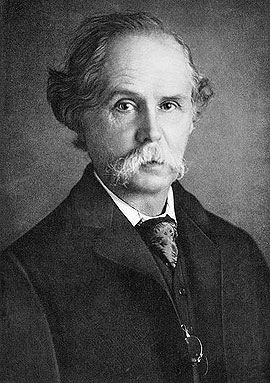
\includegraphics[width=1\textwidth]{Marshall}
     \end{center}
\end{column}
\end{columns}
\end{frame}

\begin{frame}{Эластичность}

\begin{definition}
\alert{Эластичность} $\varepsilon_{x,p}$ любой функции $x(p)$ по параметру $p$ это 
$$ \varepsilon_{x,p} = \frac{\partial \log x}{\partial \log p} = \frac{\partial x}{\partial p} \cdot \frac{p}{x}$$	
\end{definition}

Например, в Коббе-Дугласе:
$$\log x = \log I - \log p + \ldots \quad \Rightarrow \quad \varepsilon_{x,p} = -1, \ \varepsilon_{x,I} = I $$

Казалось бы, причем тут проценты?

\end{frame}

\begin{frame}{Эластичность}

Предположим, что $p,x$ как-то связаны (функционально) между собой. Рассмотрим отношение процентного изменения $x$ к процентному изменению $p$:
$$\frac{100 \delta x / x}{100 \delta p / p}=\frac{\delta x / x}{\delta p / p}$$
где $\delta x, \delta x$ – это маленькие приращения. Заметим, что:
$$=\frac{\delta x / x}{\delta p / p} \approx \frac{\log(1 + \delta x / x)}{\log(1 + \delta p / p)}=$$
далее надо вынести $x$ и $p$ из под логарифмов:
$$=\frac{\log(x + \delta x) - \log x}{\log(p + \delta p) - \log p}$$
и то, что мы получаем, – это примерно приращение логарифма $x$ относительно логарифма $p$.

\end{frame}

\begin{frame}{Эластичность}

Таким образом, мы получаем три эластичности:
$$\varepsilon_{x,p} = \frac{\partial \log x}{\partial \log p}, \quad \varepsilon_{x,q} = \frac{\partial \log x}{\partial \log q}, \quad \varepsilon_{x,I} = \frac{\partial \log x}{\partial \log I}.$$

Легко видеть, что у эластичности нет единиц измерения, так как они успешно сокращаются в правой части формулы. 

$$\varepsilon_{x,p} = \frac{\partial x}{\partial p}\frac{p}{x}, \quad \varepsilon_{x,q} = \frac{\partial x}{\partial q}\frac{q}{x}, \quad \varepsilon_{x,I} = \frac{\partial x}{\partial I}\frac{I}{x}.$$

Пользоваться можно любым из двух определений.

\end{frame}

\begin{frame}{Эластичность в данных}

Предположим что у вас есть два достаточно близких наблюдения цены: $p_1, p_2$, и два наблюдения спроса $q_1, q_2$, всю кривую спроса вы не можете видеть. Как посчитать эластичность?
	
	\begin{itemize}
	\item $\varepsilon_{p,q} = ((q_2 - q_1)/q_1)/((p_2-p_1)/p_1)$
	\item $\varepsilon_{p,q} = ((q_2 - q_1)/q_2)/((p_2-p_1)/p_2)$
	\item $\varepsilon_{p,q} = ((q_2 - q_1)/q_0)/((p_2-p_1)/p_0)$
	\end{itemize}
	
	где $p_0 = (p_1 + p_2)/2$, $q_0 = (q_1+q_2)/2$. Все они сходятся к теоретическому определению, в пределе. Последнее называется \alert{mid-point formula} в английской литературе, это сделано для того, чтобы эластичность не зависела от направления $1 \to 2$ или $2 \to 1$.
	
\end{frame}

\section{Эластичности по доходу}

\begin{frame}{Эластичности по доходу}

Для всех товаров $x,y,z$ в вашей модели вы можете определить эластичность по доходу:
$$\varepsilon_{x,I}, \quad \varepsilon_{y,I}, \quad \varepsilon_{z,I}$$

Внимание, \alert{знаки у эластичностей те же, что и у наклонов}. Поэтому, у нормальных товаров эластичности дохода положительные. Действительно:
$$\varepsilon_{x,I} = \frac{\partial x}{\partial I} \frac{I}{x}.$$

Любопытным является то, что эластичности по доходу у всех товаров связаны простым линейным соотношением, правда, разным в каждой новой точке.

\end{frame}

\begin{frame}{Эластичности по доходу}

\begin{lemma}
Всегда выполнено следующее тождество:
$$\varepsilon_{x,I} \cdot s_x + \varepsilon_{y,I} \cdot s_y + \varepsilon_{z,I} \cdot s_z = 1$$
где $s_x, s_y, s_z$ доли расходов на соответствующие товары.
\end{lemma}

Доказательство этого факта вытекает прямиком из бюджетного ограничения. Поскольку доли всегда неотрицательные, то это еще один раз показывает, что \alert{все товары не могут быть одновременно инфериорными}.

\end{frame}

\section{Эластичности по цене}

\begin{frame}{Эластичности по цене}

У каждого товара есть \alert{собственная эластичность} по цене и \alert{перекрестная эластичность} с каждым из других товаров. 

\end{frame}

\begin{frame}{Эластичности по цене}

Первым на сцену выступает, конечно же, собственная эластичность по цене:
$$\varepsilon_{x,p}, \quad \varepsilon_{y,q}, \quad \varepsilon_{z,r}.$$

Интуиция подсказывает нам, что, в принципе, собственная эластичность должна быть скорее отрицательная. Двукратное увеличение цены на товар должно, скорее всего, понизить спрос (не путать с кривой спроса) на этот товар. 

Это действительно так, кроме тех случаев, когда товар Гиффена (об этом мы поговорим подробнее в лекции 4).

\end{frame}


\begin{frame}{Эластичности по цене}
Экономисты любят говорить о спросе в терминах эластичности потребления (по собственной цене) подразумевая то, насколько товар является не критическим для существования.
\begin{center}
     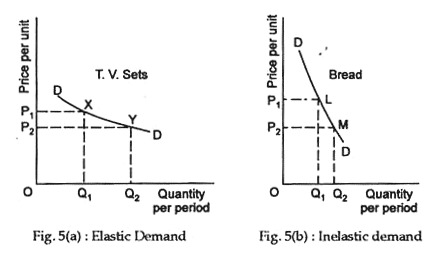
\includegraphics[width=.9\textwidth]{elast}
     \end{center}
\end{frame}

\begin{frame}{Эластичности по цене}
Как правило, глядя на сам товар, сложно сказать, насколько эластичен спрос на него, потому что это зависит от контекста а также от наличия субститутов. Например,

\begin{itemize}
  \item спрос на водный транспорт можно считать эластичным
  \item однако если вы живете на острове, то он неэластичен
  \item спрос на бензин (и энергию в целом) считается универсально неэластичным
\end{itemize}

Спрос на похоронные услуги максимально неэластичен.
\end{frame}


\begin{frame}{Эластичности по цене}

Посмотрим на собственную эластичность Кобба-Дугласа. Это очень удобная полезность для подсчета эластичности, так как мы уже привыкли везде тащить за собой логарифм.
$$\log x = \log I - \log p + \log(\alpha) - \log(\alpha + \beta + \gamma), \quad \Rightarrow \quad \varepsilon_{x,p} = -1.$$

Эластичность оказалась равна -1, то есть, она не зависит ни от цен, ни от бюджета. Это большое везение, вообще говоря эластичность не обязана быть постоянной.

\end{frame}

\begin{frame}{Эластичности по цене}

Чуть более интересным представляется анализ перекрестной эластичности, которых $n(n-1)$ штук для $n$ товаров. Это очень большое число, поэтому мы редко будем работать с $n>3$. Пусть будет три товара: $x,y,z$, тогда есть шесть эластичностей:
\begin{gather*}
\varepsilon_{x,q}, \varepsilon_{x,r}, \quad \varepsilon_{y,p}, \varepsilon_{y,r}, \quad \varepsilon_{z,p}, \varepsilon_{z,q}.
\end{gather*}

Они также называются \alert{эластичностями замещения}.

В Коб-Дугласе они все равны нулю.

\end{frame}

\begin{frame}{Эластичности по цене}

Эти эластичности хранят информацию о, грубо говоря, тенденциях к замещению между нашими товарами. Поскольку цены и спросы неотрицательны, мы можем однозначно связать знак эластичности с природой замещения между любыми двумя товарами.

Если $\varepsilon_{x,q} > 0$ то $x$ это скорее субститут по отношению к $y$. Если $\varepsilon_{x,q} < 0$ то $x$ это скорее комплемент по отношению к $y$.

Сложно сказать, что такое ноль, Кобб-Дуглас он "немножко субститут" и "немножко комплемент" одновременно, мы вернемся к этому в 4 лекции.

\end{frame}

\section{Приложения эластичности}

\begin{frame}{Эластичности по цене}

Вообще, \alert{можно мерять эластичность чего угодно}.

Одним из самых популярных приложений эластичности является анализ поведения монополиста, производящего товар, эластичность потребления которого подразумевается известной.

В то время как классическая микроэкономическая теория осписывает поведение фирм-ценополучателей, на практике, каждая фирма обладает, пусть даже очень маленькой, но рыночной властью. То есть все фирмы способны манипулировать ценой за счет снижения объемов производства, просто у монополии это получается лучше всех.

\end{frame}

\begin{frame}{Эластичности по цене}

Эластичность позволяет сделать любую из двух вещей:

\begin{itemize}
\item если вы находитесь в позиции контролирующего органа, эластичность спроса позволит вам понять, пользуется ли монополист своей рыночной властью
\item если вы находитесь в позиции истинного монополиста, эластичность спроса позволит вам установить цену, максимизирующую прибыль
\end{itemize}

Сейчас мы вкратце обсудим каждую из них.

\end{frame}

\section{Индекс Лернера}

\begin{frame}{Индекс Лернера}

Пусть на рынке установлена цена $P^{\ast}$, а маржинальные издержки (не путать с фиксированными) фирмы равны $MC$ при текущем объеме.

Назовем \alert{фиксированными издержками} $FC$ - такие издержки, которые не зависят от объема производства: получить лицензию, арендовать помещение... Назовем \alert{маржинальными издержками} $MC$ - дополнительные (или маржинальные) издержки на производство дополнительной единицы товара: сырье, электричество, труд... То есть
$$ TC(q) = FC + q \cdot MC(q),$$
где $TC$ – это общие издержки на производство $q$ единиц товара.
\end{frame}

\begin{frame}{Индекс Лернера}

Как измерить рыночную власть монополиста?

\begin{definition}
\alert{Индекс Лернера} $L$ вычисляется по формуле
$$L = \frac{P^{\ast}-MC}{P^{\ast}}$$
\end{definition}
Индекс Лернера $L$ показывает отношение маржи фирмы к действующей цене, то есть маржа в <<долях>>.

\begin{definition}
\alert{Маржа} (по-английски markup) – это 
$$P^{\ast}-MC$$
\end{definition}

\end{frame}

\begin{frame}{Индекс Лернера}

Сама по себе маржа не является злом, однако злом считается $L$. Чем больше $L$, тем более вероятно, что фирма злоупотребляет своим монопольным положением.

В Американских исследованиях <<подозрительной>> будет фирма, у которой индекс Лернера слишком высокий (граница зависят от индустрии). Такие фирмы, как правило, находятся под пристальным взглядом Федеральной Торговой Комиссии - контролирующего органа США. 

Но почему? Ответ кроется в эластичностях.

\end{frame}

\section{Формула обратной эластичности}

\begin{frame}{Формула обратной эластичности}

Пусть спрос на товар $x$ описывается \alert{обратной функцией спроса} $P(x)$ с постоянной эластичностью $\delta$, а \alert{переменные издержки} монополиста линейны и равны $MC \cdot x$. 

Заметим, что эластичность $\varepsilon$ классической кривой спроса $x(P)$ равна обратной эластичности обратной кривой спроса $1/\delta$. 

Тогда задача монополиста это:
$$ (P(x) - MC)x \to \max_x$$

\end{frame}

\begin{frame}{Формула обратной эластичности}

Используя условия первого порядка,
\begin{gather*}
P(x) - MC + P'(x)x = 0\\
(P(x) - MC)/P(x) = - P'(x)x/P(x) = - \delta
\end{gather*}

То есть, маржа/цена (то что слева) равна минус эластичности обратной функции спроса.
\end{frame}

\begin{frame}{Формула обратной эластичности}

А как это связано с (прямой) функцией спроса? Оказывается, что у обратных функций эластичность - тоже обратная. То есть 

\begin{lemma}
Если у функции спроса эластичность по цене равна $\varepsilon$, то маржа (как доля от цены) монополиста (с постоянными издержками $MC$) в оптимуме должна равняться в точности обратной эластичности с минусом:
$$\frac{P-MC}{P} = - \frac{1}{\varepsilon}$$
\end{lemma}
Конечно же, $p=MC$ – это поведение конкурентной фирмы, соответствует индексу Лернера равного в точности нулю.
\end{frame}

\section{Вернемся к CES}

\begin{frame}{Вернемся к CES}

\begin{definition}
Полезностью \alert{CES} (constant elasticity of substitution) называется
$$U(x,y) = (x^{\rho} + y^{\rho})^{1/\rho}$$
\end{definition}

Первый вопрос, который приходит нам в голову, является ли она квазивогнутой? 

Рассмотрим отдельно случаи: $\rho = 1, 2$ и $\rho < 1$.

\end{frame}

\begin{frame}{Вернемся к CES}

Утверждается, что
$$ x^{\ast}(p,q,I) = \frac{p^{\sigma}}{p^{\sigma} + q^{\sigma}} \frac{I}{p}, \quad y^{\ast}(p,q,I) = \frac{q^{\sigma}}{p^{\sigma} + q^{\sigma}} \frac{I}{q}$$

где $\sigma = \rho/(\rho-1)$.

Убедимся (i) что у нее постоянны эластичности замещения (ii) что в них выполнены условия первого порядка, а значит это оптимум. Наконец, выведем косвенную полезность.

$$V(p,q,I) = \frac{I}{(p^{\sigma}+q^{\sigma})^{\sigma}}$$
\end{frame}

\section{Квазилинейная}

\begin{frame}{Квазилинейная}

Пожалуй, третья самая важная полезность имеет следующий вид:

\begin{definition}
\alert{Квазилинейной} полезностью называется:
$$U(\vec x, y) = f(\vec x) + k y,$$ 
где $f$ - вогнутая функция.
\end{definition}

Интерпретация последней координаты - это деньги на счету. $f$ именно вогнутая, чтобы можно было прибавить к ней линейную и не сломать случайно квази-вогнутость.
\end{frame}

\begin{frame}{Квазилинейная}

Выпишем Лагранжиан:
$$\mathcal{L} = f(x) + k y - \lambda (px + y - I).$$ 
Легко, правда?

Обратите внимание, что цена денег равна единице, это стандартная нормировка в контексте квазилинейной полезности.

\end{frame}

\begin{frame}{Квазилинейная}

Сейчас мы попробуем найти внутреннее решение.

$\mathcal{L}'_x = f'_x - \lambda p = 0$

$\mathcal{L}'_y = k - \lambda = 0$

$\mathcal{L}'_{\lambda} = I - p x - y= 0$

\end{frame}

\begin{frame}{Квазилинейная}

Легко видеть, что они эквивалентны

$k = \lambda$

$x = (f')^{-1}(\lambda p)$

$px + y = I$

\end{frame}

\begin{frame}{Квазилинейная}

Однако эта система не всегда имеет решение в $\mathbb{R}^2_{+}$. Легко видеть, что спрос на товар $x$ никак не зависит от бюджета, а стало быть, при достаточно маленьком бюджете получится противоречие:
$$ x = (f')^{-1}(kp)$$

\end{frame}

\begin{frame}{Квазилинейная}

Мы оказались в неприятной ситуации. Условия первого порядка указали на точку, которая может оказаться вне допустимой области. Если это так, это значит что решение не внутреннее, а краевое. 

В таком случае, мы заменяем условие первого порядка  $x = (f')^{-1}(kp)$ на краевое условие: 
$$y=0, \quad x = I/p.$$

\end{frame}

\begin{frame}{Квазилинейная}

В этой задаче есть два взаимоисключающих режима: внутреннее решение и краевое решение. Но, если очень сильно надо, можно записать ответ в компактной форме, если проявить немного смекалки.

\end{frame}

\begin{frame}{Квазилинейная}

Спрос на каждый товар в квазилинейной полезности описывается следующими уравнениями:
\begin{gather*}
x^{\ast} = \min (I/p, (f')^{-1}(k p)), \\
y^{\ast} = \max (0, I-px^{\ast}).
\end{gather*}
Все товары в квазилинейной полезности являются нормальными.
\end{frame}

\begin{frame}{Квазилинейная}

Наконец, если решение внутреннее то
$$V(p,I) = f(x^{\ast}) + k(I - p x^{\ast}), \quad x^{\ast} = (f')^{-1}(k p).$$

Когда решение краевое то
$$V(p,I) = f(I/p).$$

\end{frame}

\section{Сумма вогнутых}

\begin{frame}{Сумма вогнутых}

Ничего не мешает нам определить полезность следующим образом:
$$ U(\vec x, \vec y) = f(\vec x) + g(\vec y)$$

где $f,g$ вогнутые функции. Пусть цены товаров $\vec p, \vec q$.

Как будет выглядеть решение такой задачи?

\end{frame}

\begin{frame}{Сумма вогнутых}

Разобъем бюджет на две части: $I_f, I_g$ и решим отдельно две оптимизационные задачи:
$$f(x) \to \max_{\vec p \cdot \vec x \leqslant I_f}, \quad g(y) \to \max_{\vec q \cdot \vec y \leqslant I_g}$$
затем найдем косвенные полезности и решим еще одну задачу:
$$V_f(p,I_f) + V_g(q,I_g) \to \max_{I_f + I_g = I} $$

\end{frame}

\begin{frame}{Сумма вогнутых}

Пример:
$$ U(x_1,x_2, y_1,y_2) =(\frac{x_1}{a} + \frac{x_2}{b}) + \alpha \log y_1 + \beta \log y_2$$
Пусть цены товаров: $p_1, p_2, q_1, q_2$.

Зная косвенные полезности наизусть, получаем:
$$ \frac{I_1}{\min(a p_1, b p_2)} + (\alpha + \beta) \log I_2 - \alpha \log q_1 - \beta \log q_2 + K$$
Осталось промаксимизировать по $I_1, I_2$ и подставить их в готовые ответы для каждой группы товаров.
\end{frame}

\begin{frame}{Метод подстановки}

Избавимся от лишних констант:
$$ \frac{I_1}{\min(a p_1, b p_2)} + (\alpha + \beta) \log I_2 \to \max_{I_1,I_2}, \quad I_1 + I_2 = I$$
Для разнообразия воспользуемся \alert{методом подстановки}:
$$ \frac{I-I_2}{\min(a p_1, b p_2)} + (\alpha + \beta) \log I_2 \to \max_{I_2}$$
Убеждаемся еще раз, что задача выпуклая, и находим оптимальные уровни бюджетов $I_1, I_2$. Потом возвращаемся в начало и доделываем задачу отдельно для каждой группы товаров.
\end{frame}

\begin{frame}{Метод подстановки}

Любая из этих задач ждет вас в домашке:

\begin{itemize}
  \item CES + уголки
  \item C-D + линейная
  \item CES + C-D
  \item уголки + линейная
  \item C-D + уголки
\end{itemize}

\end{frame}


\section{Теорема об огибающей}

\begin{frame}{Теорема об огибающей}

Это чрезвычайно важная теорема. Рассмотрим семейство опорных функций $f(x, p)$, где $x$ - переменная а $p$ - параметр. 

Определим огибающую $V(p)$ как результат оптимизации функции $f$ по какому-то статическому множеству $Х$: 
$$ V(p) := \max_{x \in X} f(x, p),$$

\begin{theorem}[Об огибающей]
Функция $V(p)$ дифференциируема (почти всюду) и 
$$\frac{\partial V(p)}{\partial p} = \frac{\partial f(x, p)}{\partial p}|_{x = x^{\ast}(p)}.$$
\end{theorem}

\end{frame}

\begin{frame}{Теорема об огибающей}

... то есть, наклон огибающей равен наклону опорной функции в точке касания.

Представьте себе, что вы сложили вместе крупные предметы разной формы (стол, компьютер, велосипед) и, чтобы они не пылились, накрыли все эластичной пленкой. 

Пленка плотно прилегла к тем предметам, которые оказались, по разным причинам выше всех остальных. Можно сказать, что пленка - это (верхняя) огибающая вашего семейства опорных объектов, поскольку она лежит там, где находится самый высокий объект в каждой точке.

\end{frame}

\begin{frame}{Теорема об огибающей}

\begin{figure}[hbt]
\centering
\includegraphics[width=.8 \textwidth]{envelope2.png}
\end{figure}

\end{frame}

\begin{frame}{Теорема об огибающей}

Запомните следующую мантру: 

\alert{наклон огибающей равен наклону опорной функции в точке касания}. 

То есть, чтобы найти наклон огибающей в точке $p$ нужно из всех опорных функций (они индексированы через $x$) выбрать ту, на которую в этой точке (точка – это значение параметра $p$) опирается огибающая, и взять ее наклон, опять же, в пространстве параметра $p$. 

\end{frame}

\begin{frame}{Теорема об огибающей}

Чтобы не перепутать, какие роли $x$ и $p$, помните, что \alert{огибающая - это функция от параметра}, а не от оптимизационной переменной, которая индексирует опорные функции. 

Соответственно, \alert{огибание происходит в пространстве параметра, а не в пространстве переменных, по которой вы оптимизировали}.

\end{frame}

\section{Практическая польза}

\begin{frame}{Теорема об огибающей}

Может показаться, что дифференцирование опорной функции и подстановка – это лишняя трата времени, ведь можно просто решить задачу и продифференцировать $V$ по параметру, в лоб.

Это правда, однако если у вас абстрактная функция, вы не можете просто так ее промаксимизировать. Поэтому эта теорема очень удобна при доказательствах, но не только. 

Более того, теорему об огибающей можно применять сразу к Лагранжиану, как минимум, в выпуклом случае (в общем случае - не уверен).

\end{frame}

\begin{frame}{Теорема об огибающей}

Рассмотрим простой пример:

Опорная функция $$ f(x|a,b) = - (x-a)^2 - b $$
Максимизируем ее $$ x^{\ast} = a, \quad f^{\ast} = - b $$
Дифференциируем истинный ответ: $$\partial f^{\ast}/\partial a = 0, \ \partial f^{\ast}/\partial b = -1$$
Дифференциируем (казалось бы, зачем?) опорную функцию: $$\partial f/\partial a = -2(x^{\ast}-a), \ \partial f/\partial b = -1$$
\end{frame}

\begin{frame}{Теорема об огибающей}

Рассмотрим пример посложнее:

Опорная функция Кобб-Дуглас $$ f(x|a,b) = \alpha \log x + \beta \log y - \lambda (px + qy - I) $$
Вы хотите найти наклон косвенной полезности, но забыли формулу. Однако, вы помните формулу оптимальных координат.
Дифференциируем опорную функцию: $$\partial f/\partial \alpha = \log x^{\ast}, \ \partial f/\partial \beta = \log y^{\ast}, \ \partial f/\partial I = \lambda^{\ast}$$
Не забываем подставить оптимальные $x^{\ast}, y^{\ast}, \lambda^{\ast}$.
\end{frame}

\begin{frame}{Теорема об огибающей}

Вопрос на засыпку: 

Если $V$ косвенная полезность, то чему равна $\partial V/ \partial I$?
\end{frame}

\begin{frame}{Теорема об огибающей}
Она равна множителю Лагранжа $\lambda$.

В частности, это может помочь вам быстро найти $\lambda$, если вас попросят в домашке вычислить его.
\end{frame}

\section{Минимизация расходов}

\begin{frame}{Минимизация расходов}
Сейчас мы перейдем к задаче, на первый взгляд, никак не связанной с максимизацией полезности. Если быть точными, мы будем минимизировать сумму расходов на все товары при минимально заданном таргетированном уровне полезности $\bar U$. 

Для простоты пусть будут два товара $x, y$ с ценами $p, q$. 
$$\text{P2:} \quad p x + q y \to \min_{x,y \geqslant 0}, \quad \text{s.t.} \quad U(x,y) \geqslant 0.$$

Сравните с классической задачей максимизации полезности
$$\text{P1:} \quad U(x, y) \to \max_{x,y \geqslant 0}, \quad \text{s.t.} \quad p x + q y \leqslant 0.$$
\end{frame}

\begin{frame}{Минимизация расходов}
Сравним лагранжианы
\begin{gather*}
\mathcal{L}^{1} = U(x, y) - \lambda (px + qy - I)\\
\mathcal{L}^{2} = (px + qy - I) - \gamma (\bar U - U(x,y))
\end{gather*}

Сравним фоки (упп)
\begin{gather*}
\text{P1:} \quad U'_x = \lambda p, \quad U'_y = \lambda q, \quad px + qy = I\\
\text{P2:} \quad p = \gamma U'_x, \quad q = \gamma U'_y, \quad U(x,y) = \bar U
\end{gather*}

Решения совпадают, если третьи уравнения эквивалентны.

Это свойство известно как Закон Вальраса.
\end{frame}

\section{Закон Вальраса}

\begin{frame}{Закон Вальраса}

Для начала приведем пример полезности, при которой Закон Вальраса не выполнен, это постоянная полезность $U(x,y) = 1$. 

Действительно, с точки зрения полезности все бюджетное множество состоит из оптимумов. Однако лишь одна точка $(x,y)=(0,0)$ по настоящему минимизирует издержки, при таргетированной полезности $\bar U = 0$. 

Что тут произошло? Дело в том, что у полезности $U(x,y) = 1$ толстые линии уровня. 

Чтобы Закон Вальраса заработал, необходимо исключить появление таких линий уровня, то есть, локальная ненасыщаемость в $\mathbb{R}^2_{+}$.

\end{frame}

\begin{frame}{Закон Вальраса}

\begin{theorem}[Закон Вальраса]
Если полезность локально ненасыщаема в $\mathbb{R}^n_{+}$, то любое из решений задачи максимизации полезности всегда лежит на бюджетном ограничении.
\end{theorem}

Это утверждение доказывается от противного. 

Пусть решение находится в бюджетном множестве, но не на бюджетной линии. Тогда существует точка в его окрестности, которая также содержится в бюджетном множестве (поскольку локальная ненасыщаемость именно в $\mathbb{R}^n_{+}$), но дает большую полезность. Противоречие.

\end{frame}

\section{Два спроса}

\begin{frame}{Два спроса}

\begin{definition}
Назовем \alert{Хиксианским спрос} в задаче минимизации расходов, и \alert{Маршаллианским спрос} в задаче максимизации полезности. 
\end{definition}

Для товаров $x,y$ будем обозначать Хиксианские спросы как 
$$h_x(p,q,\bar U), \quad h_y(p,q,\bar U),$$
а Маршаллианские спросы как
$$m_x(p,q,I), \quad m_y(p,q,I).$$
Но главное - это аргументы. Какие аргументы такой и спрос.

\end{frame}

\begin{frame}{Два спроса}

Тогда в для задачи максимизации полезности с параметрами $(p,q,I)$ существует 
$$ \bar U_0 := V(m_x(p,q,I), m_y(p,q,I))$$

такой, что задача минимизации расходов с $(p, q, \bar U_0)$ эквивалентна ей. 

Аналогично, для задачи миимизации расходов с $(p, q, I)$ существует
$$ I_0 := p h_x(p,q, \bar U) + q h_y(p,q, \bar U)$$
такой, что задача максимизации полезности с $(p, q, I_0)$ эквивалентна ей. 

\end{frame}

\section{Дуальность}

\begin{frame}{Дуальность}

Мы подошли к очень важному наблюдению.

\begin{theorem}[Дуальность]

Если полезность (квази-)вогнутая и локально ненасыщаемая, то любое решение (как функция от цен) задачи минимизации расходов воспроизводится как одно из решений максимизации полезности и наоборот.
\end{theorem}
Причем, все это при одних и тех же ценах. Это чуть более сильное утверждение чем просто закон Вальраса.

\end{frame}

\begin{frame}
Это значит, что задача максимизации полезности и задача минимизации расходов по большому счету эквивалентны в определенном геометрическом смысле. 

Есть только одна проблема - у Маршаллианского и Хиксианского спросов разный набор аргументов, поэтому они не могут совпадать номинально. 

Для того, чтобы поправить ситуацию, нам понадобится еще одна новая функция.
\end{frame}

\section{Функция расходов}

\begin{frame}{Функция расходов}

\begin{definition}
Назовем \textbf{функцией расходов} значение целевой функции в оптимуме в задаче минимизации расходов:
$$ E(p,q,\bar U) = p h_x(p,q,\bar U) + q h_y(p,q,\bar U).$$
\end{definition}

Это совершенно аналогично тому, как мы ввели косвенную полезность $V(p,q,I)$ через значение целевой функции в оптимуме в задаче максимизации полезности.
\end{frame}

\section{Лемма Шепарда}

\begin{frame}{Лемма Шепарда}

Что произойдет, если мы применим Теорему об Огибающей к задаче минимизации расходов?
$$ -E(p,q,\bar U) = - p h_x(p,q,\bar U) - q h_y(p,q,\bar U)$$
Сперва легким движением руки заменяем минимум функции $E$ на максимум функции $-E$, тогда:
$$\frac{\partial E}{\partial p} = -\frac{\partial(-E)}{\partial p} = ?$$
\end{frame}

\begin{frame}{Лемма Шепарда}

Далее мы должны ответить на следующий вопрос:

Что есть опорная функция для $E(p,q,I)$?
\end{frame}

\begin{frame}{Лемма Шепарда}
Правильный ответ – это Лагранжиан 
$$\mathcal{L}=px + qy - \lambda(\bar U - U(x,y))$$
это опорная функция. 

Чему равен ее градиент \alert{по ценам}?

А с точки зрения Теоремы об Огибающей?
\end{frame}

\begin{frame}{Лемма Шепарда}
\begin{theorem}[Лемма Шепарда]
Если $\vec{h}$ - весь вектор спросов, а $\vec{p}$ - весь вектор цен то
$$\vec{h} = \nabla_{\vec{p}} E,$$
то есть Хиксианский спрос является градиентом (по ценам, но не бюджету) от функции расходов.
\end{theorem}

\end{frame}

\section{Тождество Роя}

\begin{frame}{Тождество Роя}

Воспользуемся дуальностью:
$$U = V(p, q, E(p,q,U)).$$
Убедитесь, что это действительно корректная запись.

Что можно сделать с этим тождеством?
\begin{itemize}
\item продифференцировать по $p$
\item продифференцировать по $q$
\end{itemize}

\end{frame}

%%%%%%%%%%%%%%%%

\begin{frame}{Тождество Роя}
Заметим, что цены входят справа дважды:
$$U = V(p, q, E(p,q,U)).$$
По правилам дифференцирования, полный дифференциал функции $V$ по $p$ равен:
\begin{gather*}
\frac{d V}{d p} = \frac{\partial V}{\partial p} + \frac{\partial V}{\partial I} \cdot \frac{\partial E}{\partial p} = 0
\end{gather*}

\end{frame}

\begin{frame}{Тождество Роя}
Поскольку $\frac{\partial E}{\partial p} = x$, 
$$\frac{d V}{d p} = \frac{\partial V}{\partial p} + \frac{\partial V}{\partial I} \cdot x_1 = 0$$
Aналогично для второй цены
$$\frac{d V}{d q} = \frac{\partial V}{\partial q} + \frac{\partial V}{\partial I} \cdot x_2 = 0$$
Комбинируя это в векторной форме, мы получаем:

\begin{theorem}[Тождество Роя]
Если $\vec{x}$ - весь вектор спросов, а $\vec{p}$ - весь вектор цен то
$$\vec{x} = - \frac{\nabla_{\vec{p}} V}{\partial V / \partial I } $$
\end{theorem}

\end{frame}

\section{Как не запутаться?}

\begin{frame}{Как не запутаться?}

Подводя итог, у нас было две задачи: максимизации полезности и минимизации расходов. Каждая задача имела свой набор параметров: первая $(p,q,I)$ а вторая $(p,q,\bar U)$. 

Каждая задача произвела три обьекта:

\begin{itemize}
\item оптимальные $m_x(p,q,I), m_y(p,q,I)$ и косвенная полезность $V(p,q,I)$ в первой задаче
\item оптимальные $h_x(p,q,\bar U), h_y(p,q,\bar U)$ и функция расходов $E(p,q,\bar U)$ во второй задаче
\end{itemize}
Можно изобразить <<схему перемещений>> между объектами

\end{frame}

\begin{frame}{Как не запутаться?}

\begin{figure}[hbt]
\centering
\includegraphics[width=.9\textwidth]{scheme.png}
\end{figure}

\end{frame}

\section{Решаем примеры до упора}

\end{document}